% -- LaTeX rewrite of main.typ, using the OUP template and matching the structure and content --

\documentclass[unnumsec,webpdf,contemporary,large]{oup-authoring-template}
\usepackage{booktabs}
\usepackage{placeins}
\usepackage{float}

\theoremstyle{thmstyleone}%
\newtheorem{theorem}{Theorem}%
\newtheorem{proposition}[theorem]{Proposition}%
\theoremstyle{thmstyletwo}%
\newtheorem{example}{Example}%
\newtheorem{remark}{Remark}%
\theoremstyle{thmstylethree}%
\newtheorem{definition}{Definition}

\begin{document}

\journaltitle{Oxford University Press.}
\copyrightyear{2025}
\appnotes{Paper}

\firstpage{1}
\setlength{\parindent}{0pt}
\setlength{\parskip}{0em}

\title[Short Article Title]{Assessing the Reliability of AlphaFold3 Predictions for Protein-Ligand Affinity Prediction via Sfcnn}

\author[1]{Guo Yu}
\author[1]{Yiming Wu}
\author[1]{Yiyang Tan}

\authormark{Guo Yu et al.}

\address[1]{\orgdiv{School of Information Science and Technology}, 
\orgname{ShanghaiTech University}, 
\orgaddress{\street{393 Middle Huaxia Road}, \postcode{201210}, \state{Shanghai}, \country{China}}}

\abstract{
This study systematically evaluates the reliability of AlphaFold3 (AF3)-predicted protein structures for protein-ligand affinity (PLA) prediction tasks. The Sfcnn model, a 3D convolutional neural network (CNN) for PLA prediction, was reproduced using PyTorch. Model performance was validated on the PDBbind v2019 refined set for training and the CASF-2016 core set for testing. Subsequently, AF3-derived protein structures from the CASF-2016 core set were assessed and compared to experimentally determined structures using Sfcnn scores, to determine the suitability of AF3 predictions in PLA applications.
}
\keywords{AlphaFold3, protein-ligand affinity, CNN scoring function, CASF-2016}

\maketitle

\section{Introduction}
\vspace{0.5em}
\subsection{Background}
AlphaFold3 (AF3), DeepMind’s latest AlphaFold model, predicts protein and protein–ligand structures with high accuracy. It extends AlphaFold2 by adding explicit ligand modeling, enhanced multimer assembly support, and optimized MSAs via deep neural networks trained on extensive sequence and structural data~\cite{AF3}.

Sfcnn is a 3D convolutional neural network-based scoring function introduced by Wang et al.~\cite{Sfcnn} in 2022, designed to provide accurate and reliable predictions of binding affinities for protein-ligand complexes.
\vspace{0.5em}
\subsection{Objective}
The primary objective of this study is to evaluate the reliability of AlphaFold3-predicted protein-ligand complex structures for protein-ligand affinity (PLA) prediction. Using the Chai-1 server for AF3 structure generation, we ensure support for custom ligands and robust MSA construction. The resulting AF3 structures are assessed with the reproduced Sfcnn model and predicted affinities are compared to those from experimentally determined structures. This enables a direct evaluation of AF3's suitability for PLA prediction and highlights its current strengths and limitations.

\section{Materials and Methods}
\vspace{0.5em}
\subsection{Datasets}
The Sfcnn network was trained using protein-ligand complexes from the PDBbind v2019 refined set\cite{Wang2005PDBbind}, which includes experimentally determined binding affinities (pKa values). The model was evaluated on the CASF-2016~\cite{su2018comparative} core set, comprising 285 protein-ligand complexes. To prevent data leakage, 266 overlapping protein complexes between the training and test sets were excluded, resulting in 4,852 unique training complexes.

\subsection{Data Augmentation}
To increase the effective size of the training set, each protein-ligand complex was randomly rotated nine times using random rotation matrices, yielding ten variants per complex. All variants share the same PLA score, resulting in a total of 48,520 training samples.

\subsection{Featurization}
Protein-ligand complexes are represented as 3D grids of size $20 \times 20 \times 20$, with each grid cell encoded as a one-hot vector of length 28. This vector comprises 14 protein atom types\footnote{\url{https://bmcbioinformatics.biomedcentral.com/articles/10.1186/s12859-022-04762-3}} and 14 ligand atom types. The resulting training tensor has shape $(48520, 20, 20, 20, 28)$.

\begin{figure}[H]
    \centering
    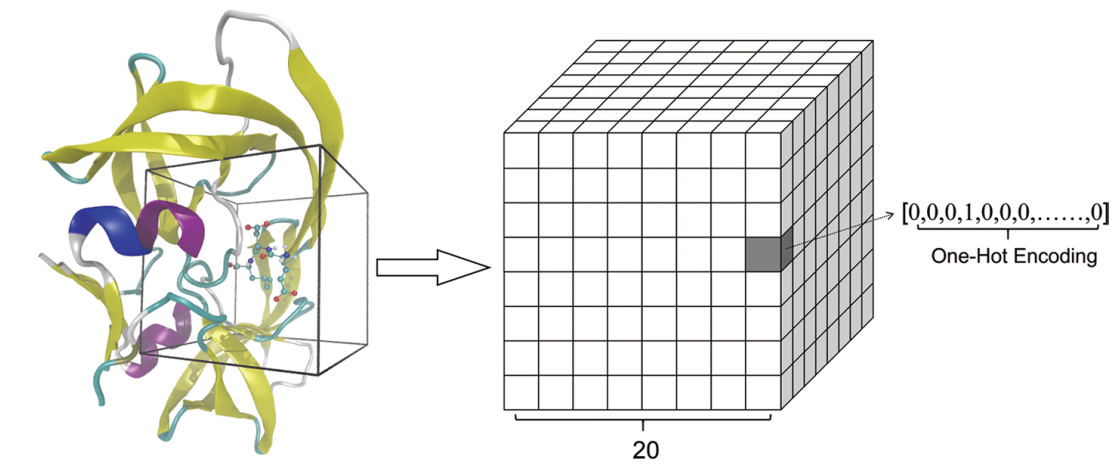
\includegraphics[width=0.5\textwidth]{images/one_hot.png}
    \caption{Featurization of protein-ligand complexes. Example shown: PDB ID 1a30. Default resolution is $20\times20\times20$ with 28 atomic categories.}
    \label{fig:onehot}
\end{figure}

\section{Sfcnn Network Architecture and Implementation}

\subsection{Architecture}
The original Sfcnn publication describes four network architectures and three featurization strategies. The architecture depicted in Figure~\ref{fig:CNN}, combined with the aforementioned featurization, achieved optimal validation performance.

\begin{figure}[H]
    \centering
    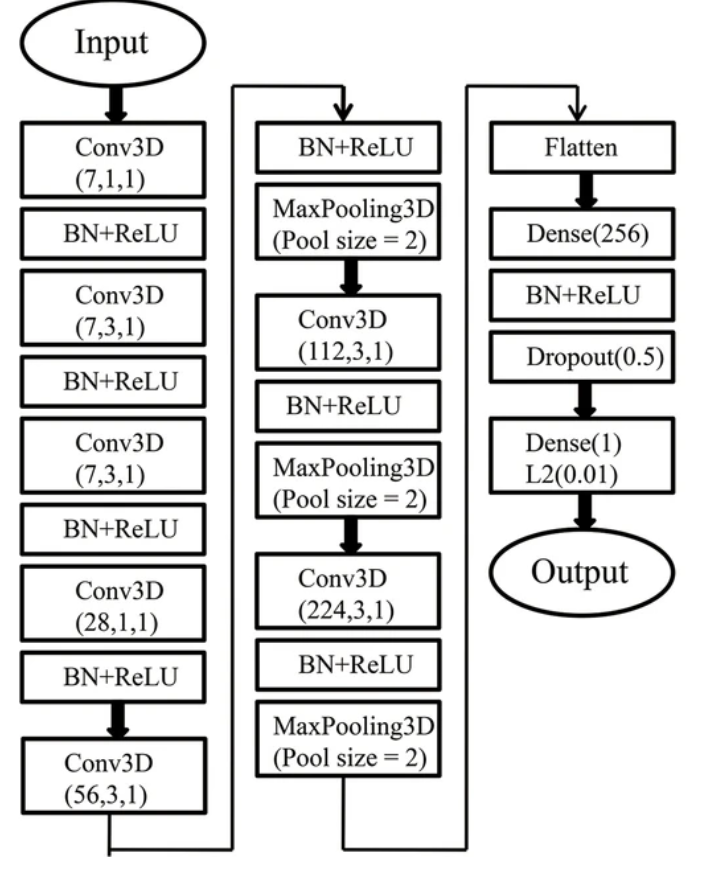
\includegraphics[width=0.35\textwidth]{images/CNN.png}
    \caption{Final CNN architecture for the Sfcnn network.}
    \label{fig:CNN}
\end{figure}

This architecture employs 3D convolutional layers with batch normalization and ReLU activation. L2 regularization is applied to the output layer to mitigate overfitting and enhance generalization.

\subsection{Implementation Details}
The PyTorch implementation closely mirrors the original TensorFlow version, with two key differences:
\begin{enumerate}
    \item Due to PyTorch's \texttt{Conv3D} API, input tensors are permuted to shape (batch\_size, 28, 20, 20, 20).
    \item PyTorch lacks a direct L2 regularization API; instead, weight decay is applied to the final fully connected layer to approximate this effect.
\end{enumerate}

\subsection{Data Storage}
The original Sfcnn implementation stored data as concatenated arrays in a single \texttt{.pkl} (pickle) file, requiring all data to reside in memory, which is impractical for extremely large datasets. The format of \texttt{.h5} (HDF5) via \texttt{h5py} is adopted for incremental writing and efficient storage. The resulting training grid occupies 40.1 GiB.

\subsection{Training Procedure}
Training and validation sets are partitioned as in the original study, with the validation set comprising indices 41,000 to 48,520. The resulting splits are: training $(41,000, 20,20,20,28)$, validation $(7,520, 20,20,20,28)$, and test $(285, 20,20,20,28)$, corresponding to a ratio of 84.00\% : 15.42\% : 0.58\%. 

Note that the original hyperparameters did not yield convergence in our PyTorch experiments. Both sets of hyperparameters are summarized below.

\begin{table}[H]
\centering
\caption{Original and Reproduced Hyperparameters}
\label{tab:hyperparams}
\begin{tabular}{lcc}
\toprule
Parameter & Original & Reproduced \\
\midrule
Learning rate & 0.004 & 0.00068 \\
Batch size & 64 & 32 \\
Dropout rate & 0.5 & 0.15 \\
L2 regularization / FC weight decay & 0.01 & 0.01 \\
Epochs & 200 & 400 \\
\bottomrule
\end{tabular}
\end{table}

\section{Reproduced Results}
\label{sec:ReproducedResults}

\subsection{Evaluation Metrics}
Sfcnn performance is evaluated using the following metrics:

\begin{align*}
\mathrm{RMSE} &= \sqrt{\frac{1}{N} \sum_{i=1}^{N} (y_{\text{predict}} - y_{\text{true}})^2} \\
\mathrm{MAE} &= \frac{1}{N} \sum_{i=1}^{N} |y_{\text{predict}} - y_{\text{true}}| \\
\mathrm{SD} &= \sqrt{\frac{1}{N-1} \sum_{i=1}^{N} ((a y_{\text{predict}} + b) - y_{\text{true}})^2} \\
\mathrm{R} &= \frac{\mathbb{E}[(y_{\text{predict}} - \mu_{y_{\text{predict}}})(y_{\text{true}} - \mu_{y_{\text{true}}})]}{\sigma_{y_{\text{predict}}} \sigma_{y_{\text{true}}}}
\end{align*}

where $a$ and $b$ are the slope and intercept of the linear regression between predicted and measured values, $\mathbb{E}[\cdot]$ denotes expectation, and $\mu$ and $\sigma$ represent means and standard deviations, respectively.

\begin{table}[H]
\centering
\caption{Performance Metrics on CASF-2016 Core Set}
\label{tab:metrics}
\begin{tabular}{lcc}
\toprule
Metric & Reproduced Sfcnn & Original Sfcnn \\
\midrule
Pearson R & 0.7678 & 0.7928 \\
RMSE & 1.4647 & 1.3263 \\
MAE & 1.1633 & 1.0277 \\
SD & 1.3928 & 1.3252 \\
\bottomrule
\end{tabular}
\end{table}

Although the original Sfcnn reports superior metrics, its training process did not converge in the reproduction, raising concerns regarding the reproducibility of the reported performance. 
Due to the lack of access to the original training data and the absence of author response to data requests on GitHub\footnote{\url{https://github.com/bioinfocqupt/Sfcnn/issues/1}}, the original training process is deemed irreproducible.

The training, validation, and testing results for the four metrics are presented in Figure~\ref{fig:ReproducedPlot} and Figure~\ref{fig:OriginalPlot}.

\begin{figure}[H]
    \centering
    \begin{minipage}{0.45\textwidth}
        \centering
        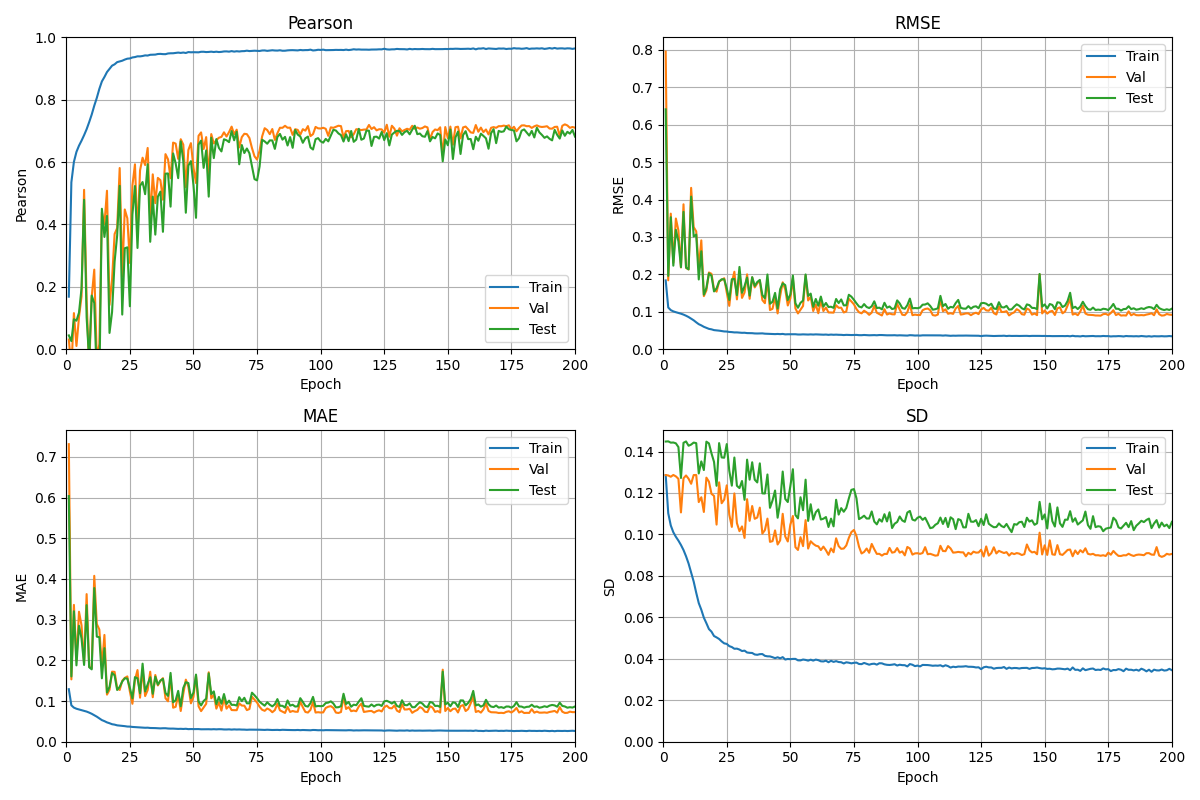
\includegraphics[width=\textwidth]{images/normal_converge.png}
        \caption{Training curve for reproduced hyperparameters.}
        \label{fig:ReproducedPlot}
    \end{minipage}\hfill
    \begin{minipage}{0.45\textwidth}
        \centering
        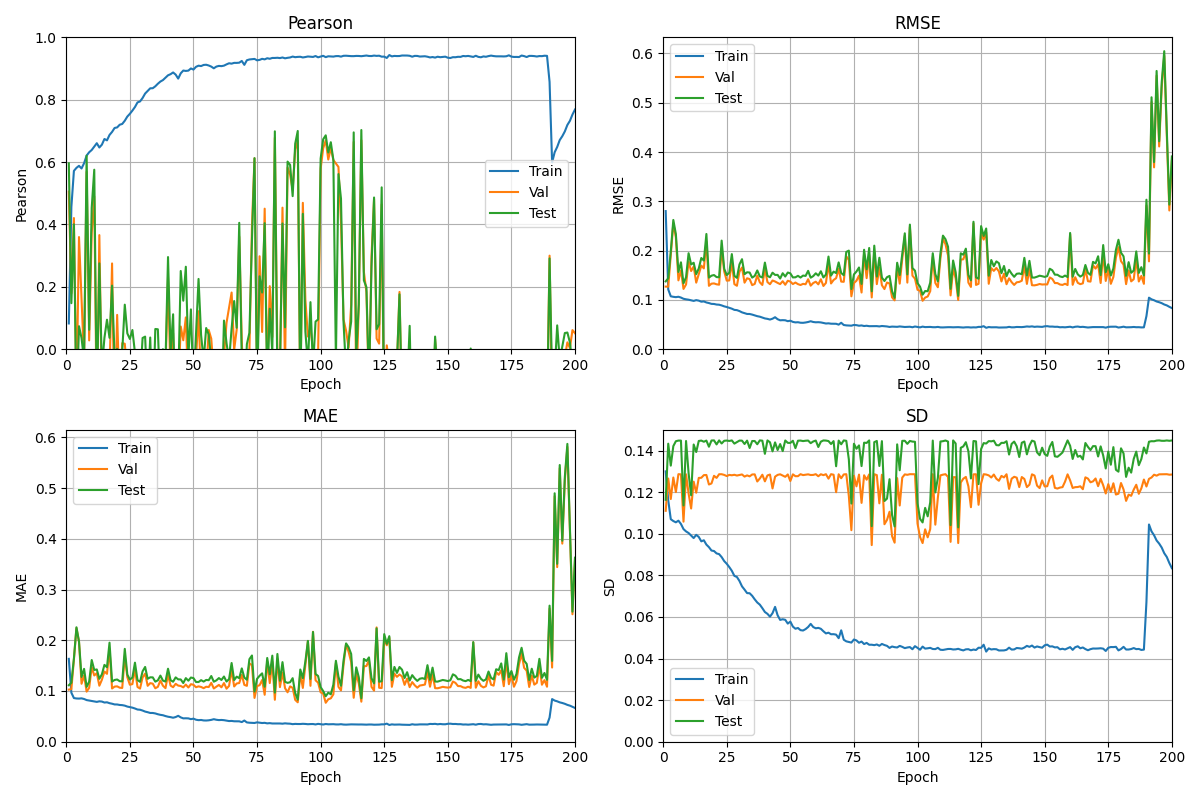
\includegraphics[width=\textwidth]{images/origin_param.png}
        \caption{Training curve for original hyperparameters.}
        \label{fig:OriginalPlot}
    \end{minipage}
\end{figure}

We conjuctured that the divergent result is caused by unusually high learning rate and drop out rate,
the reproduced results are therefore considered the baseline for subsequent AF3 result assessment.

\section{AlphaFold3 Structure Assessment}

\subsection{Dataset Selection}
The assessment utilizes the CASF-2016 core set, excluding six proteins with structural complexity beyond AlphaFold3's predictive capacity, resulting in 279 proteins. Proteins with more than five isomorphic or heterogeneous chains were excluded, as detailed in Table~\ref{tab:complex}.

\begin{table}[H]
\centering
\caption{Excluded Complex Protein Structures}
\label{tab:complex}
\begin{tabular}{lc}
\toprule
PDB ID & Number of Chains \\
\midrule
2xb8 & 12 \\
2ymd & 10 \\
3n76 & 12 \\
3n7a & 12 \\
3n86 & 12 \\
4ciw & 12 \\
\bottomrule
\end{tabular}
\end{table}

\subsection{Structure Generation and Processing}
Protein structures were generated using the \textit{Chai-1 online server}\footnote{\url{https://lab.chaidiscovery.com/dashboard}}. The AlphaFold3 online server\footnote{\url{https://alphafoldserver.com/}} was not used due to its inability to accept specific ligand SMILES codes. The MSA (Multiple Sequence Alignment) option was enabled with the MMseqs2 algorithm for all generations.

Server outputs were downloaded as zip archives containing multiple ranked structures and associated metrics. The top-ranked structure (\texttt{pred.rank\_0.cif}) was selected for analysis. To avoid conversion errors between file formats (.cif, .pdb, .mol2), structures were parsed directly using the \texttt{MMCIFParser} from the \texttt{Bio.PDB} Python package, followed by featurization and grid mapping.

Atoms or isotopes not included in the 14 predefined atom types are categorized as \texttt{other}.

\subsection{Scoring Protocol}
To quantitatively assess the reliability of AlphaFold3 (AF3)-predicted structures 
for protein-ligand affinity (PLA) prediction, we evaluated the predicted complexes 
using the reproduced Sfcnn network, initialized with pre-trained weights 
(Pearson $R = 0.768$). The experimentally determined PLA values from the PDBbind 
v2019 core set served as the ground truth. 
For benchmarking, the predicted scores for AF3-generated structures are compared 
against both the ground truth and the Sfcnn scores obtained from experimentally 
resolved structures, employing the same evaluation metrics as 
in Section~\ref{sec:ReproducedResults}.

\begin{table}[H]
\centering
\caption{Performance metrics for AF3-predicted structures compared to ground truth and Sfcnn predictions on the core set.}
\label{tab:af3_metrics}
\begin{tabular}{lcc}
\toprule
Metric & Ground Truth & Core Set Sfcnn \\
\midrule
Pearson $R$ & 0.3558 & 0.4415 \\
RMSE        & 2.0484 & 1.1366 \\
MAE         & 1.6616 & 0.9031 \\
SD          & 2.0356 & 1.0665 \\
\bottomrule
\end{tabular}
\end{table}

As summarized in Table~\ref{tab:af3_metrics}, the correlation between predicted and experimental affinities decreases when using AF3-generated structures (Pearson $R = 0.3558$) compared to experimentally determined structures (Pearson $R = 0.4415$). Both RMSE and MAE are notably higher for AF3 predictions, indicating increased prediction error and reduced model reliability on these structures.

\subsection{Error Analysis and Visualization}
To further dissect the sources and distribution of prediction errors, 
a series of visual analyses are presented below:

\begin{figure}[H]
    \centering
    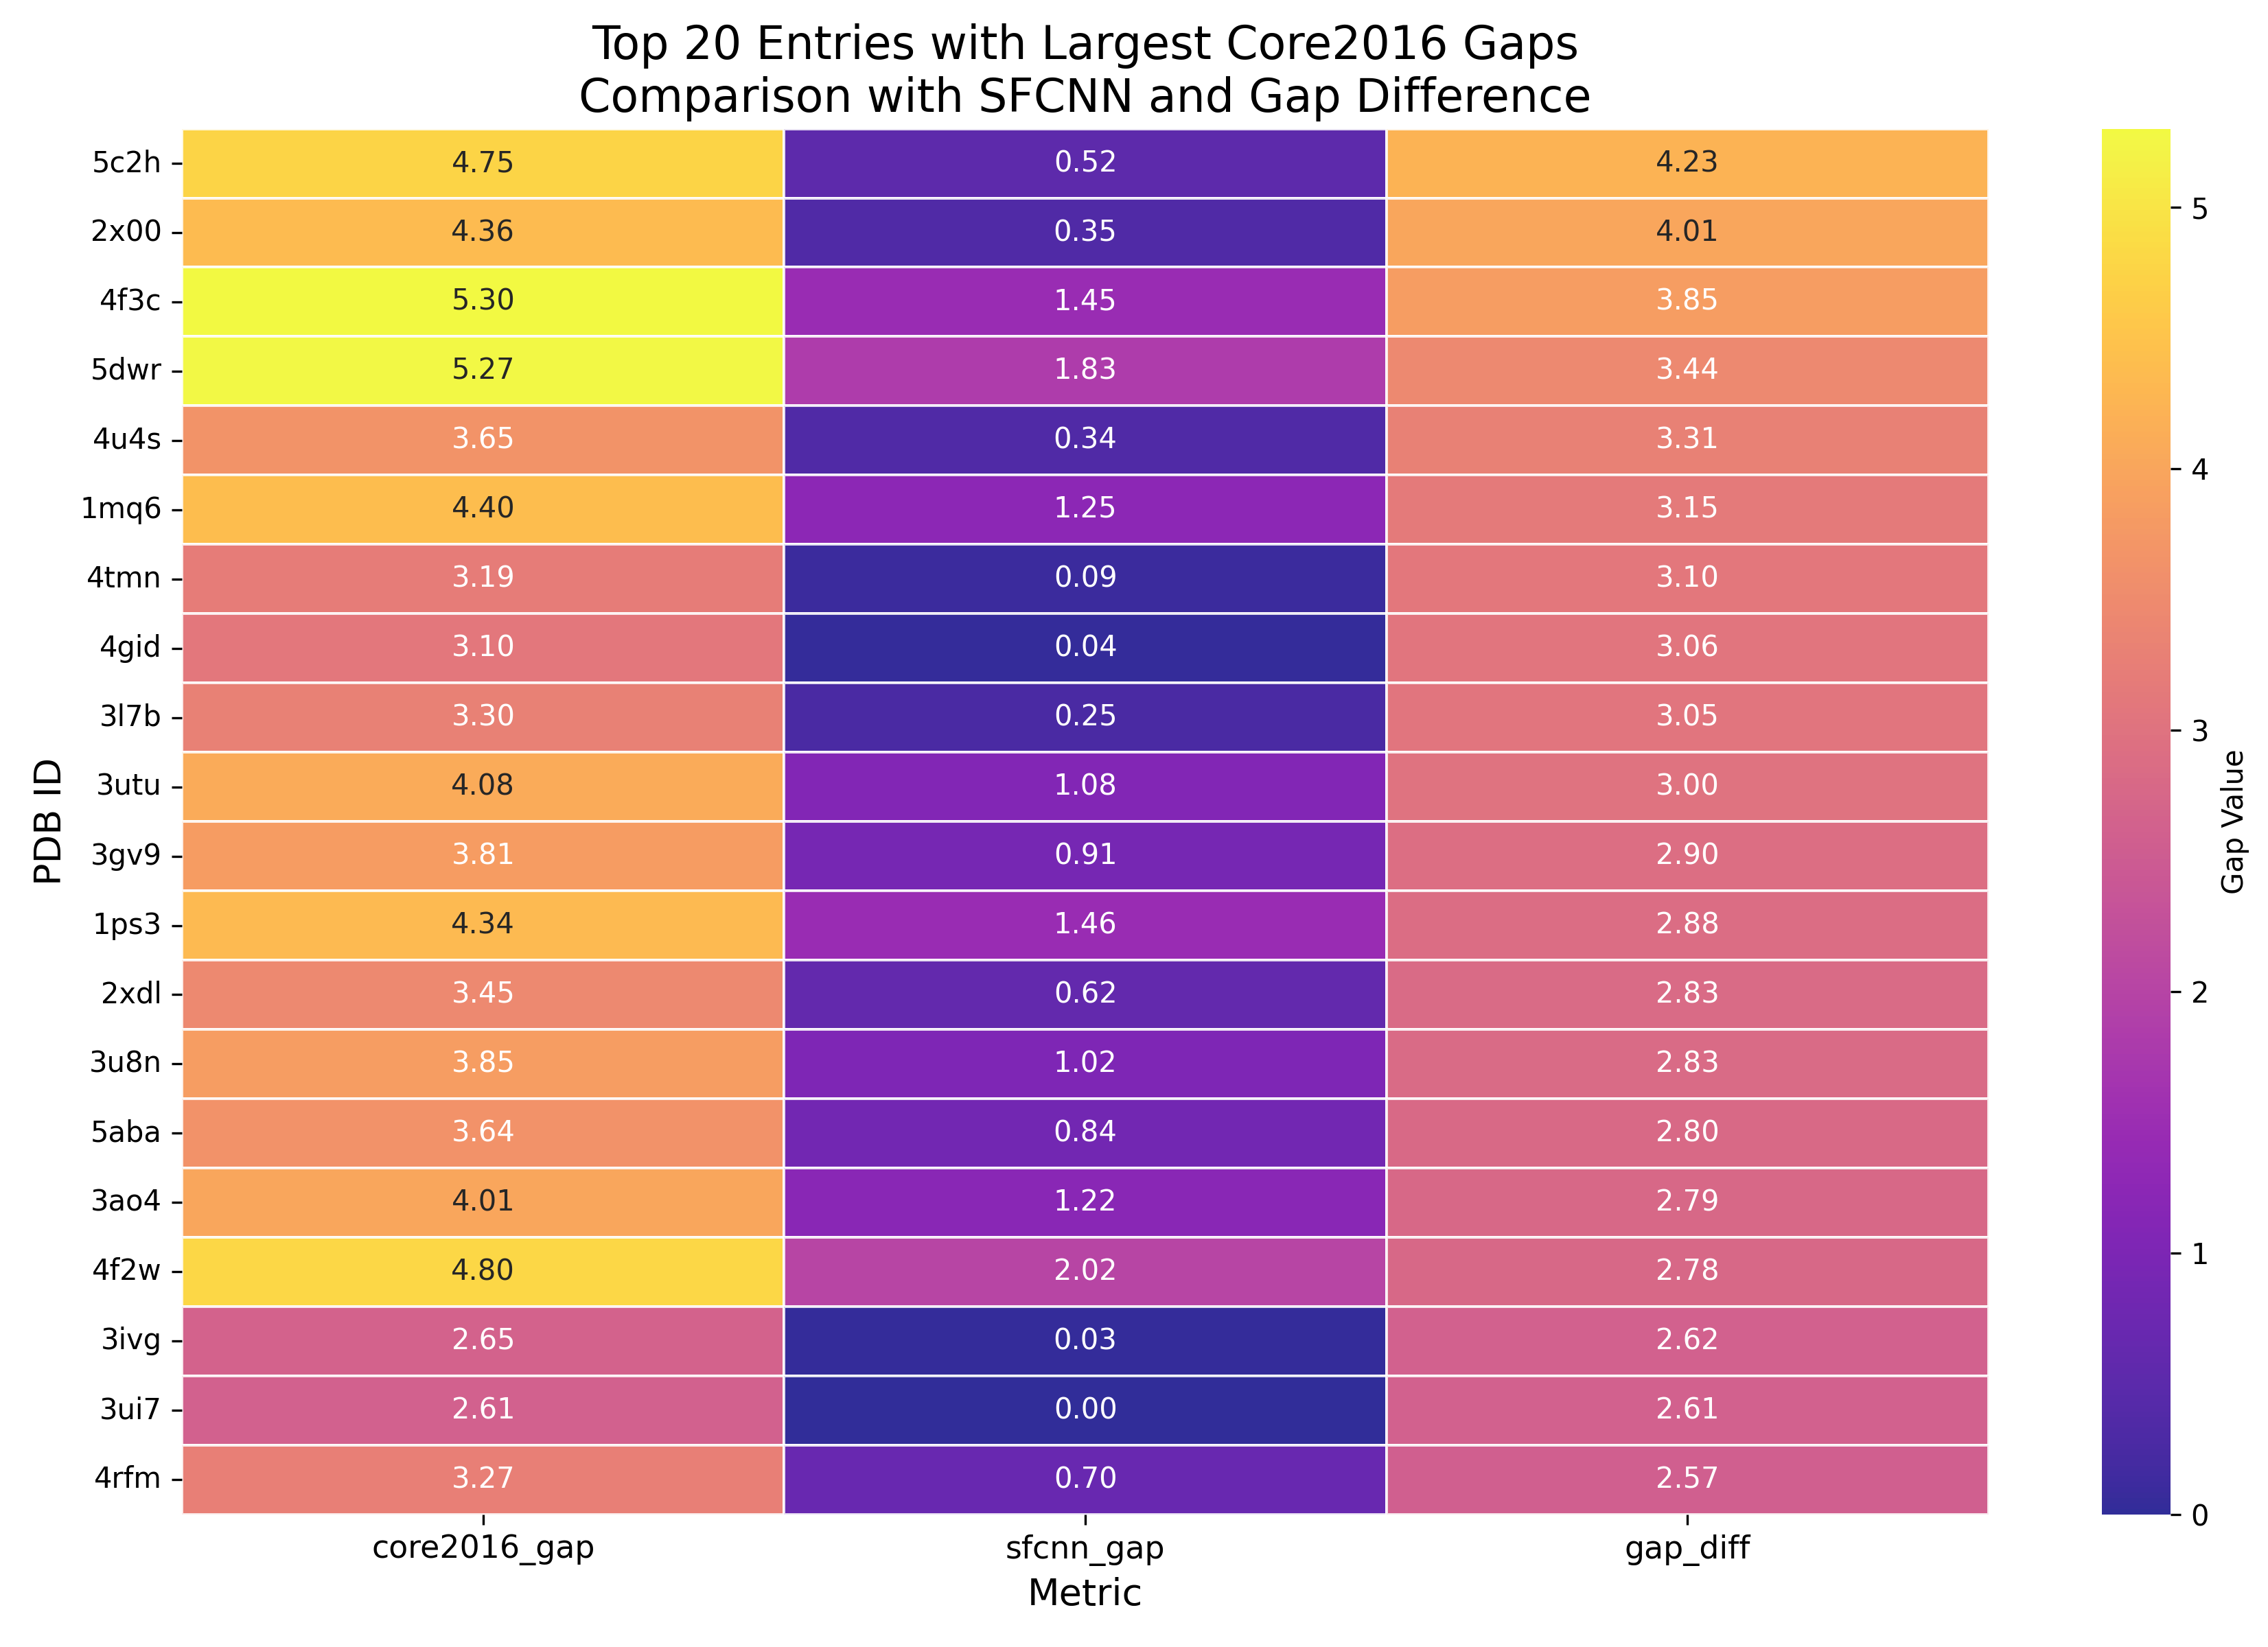
\includegraphics[width=0.34\textwidth]{images/top20_heatmap.png}
    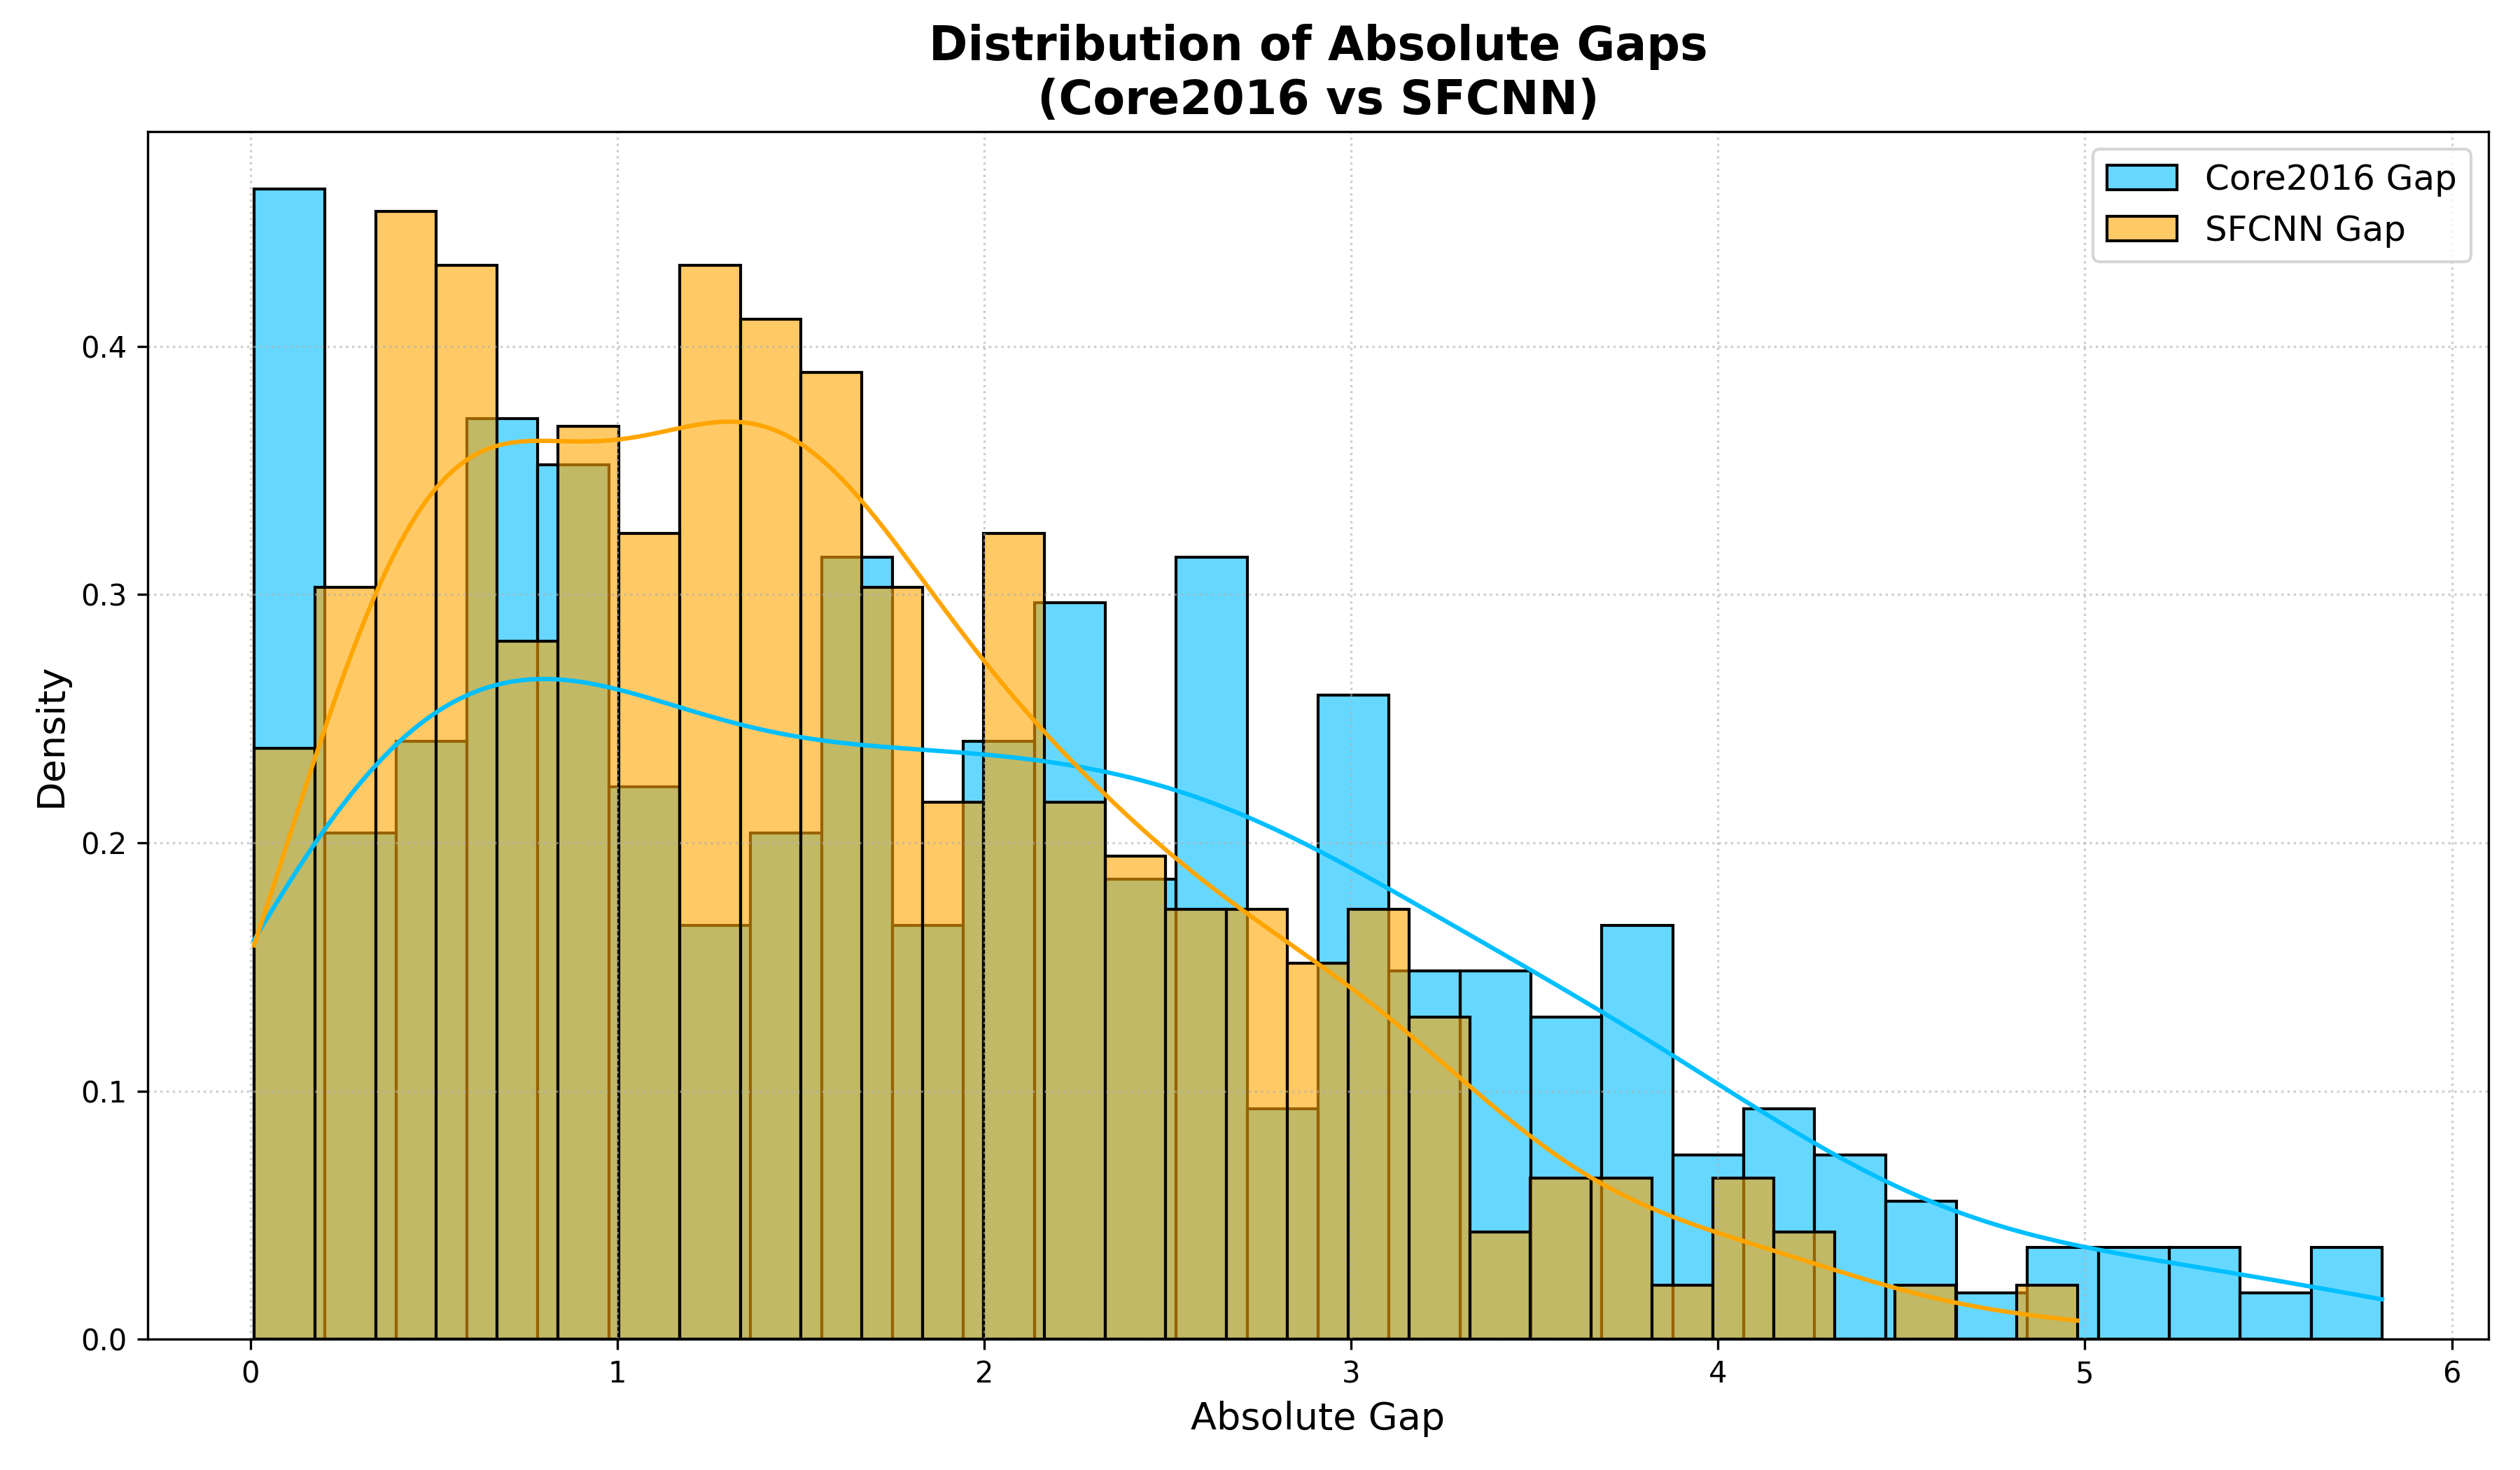
\includegraphics[width=0.34\textwidth]{images/gap_histogram.png}
    \caption{Heatmap (top) of the top 20 complexes with largest prediction gaps and histogram (bottom) of absolute prediction gaps for AF3 structures.}
    \label{fig:af3_heatmap_hist}
\end{figure}

Figures~\ref{fig:af3_heatmap_hist} illustrate the distribution and magnitude of prediction errors. The heatmap highlights complexes with the largest discrepancies between AF3-predicted and ground truth PLA scores, while the histogram reveals a right-skewed error profile, indicating that a substantial fraction of complexes exhibit large deviations.

\begin{figure}[H]
    \centering
    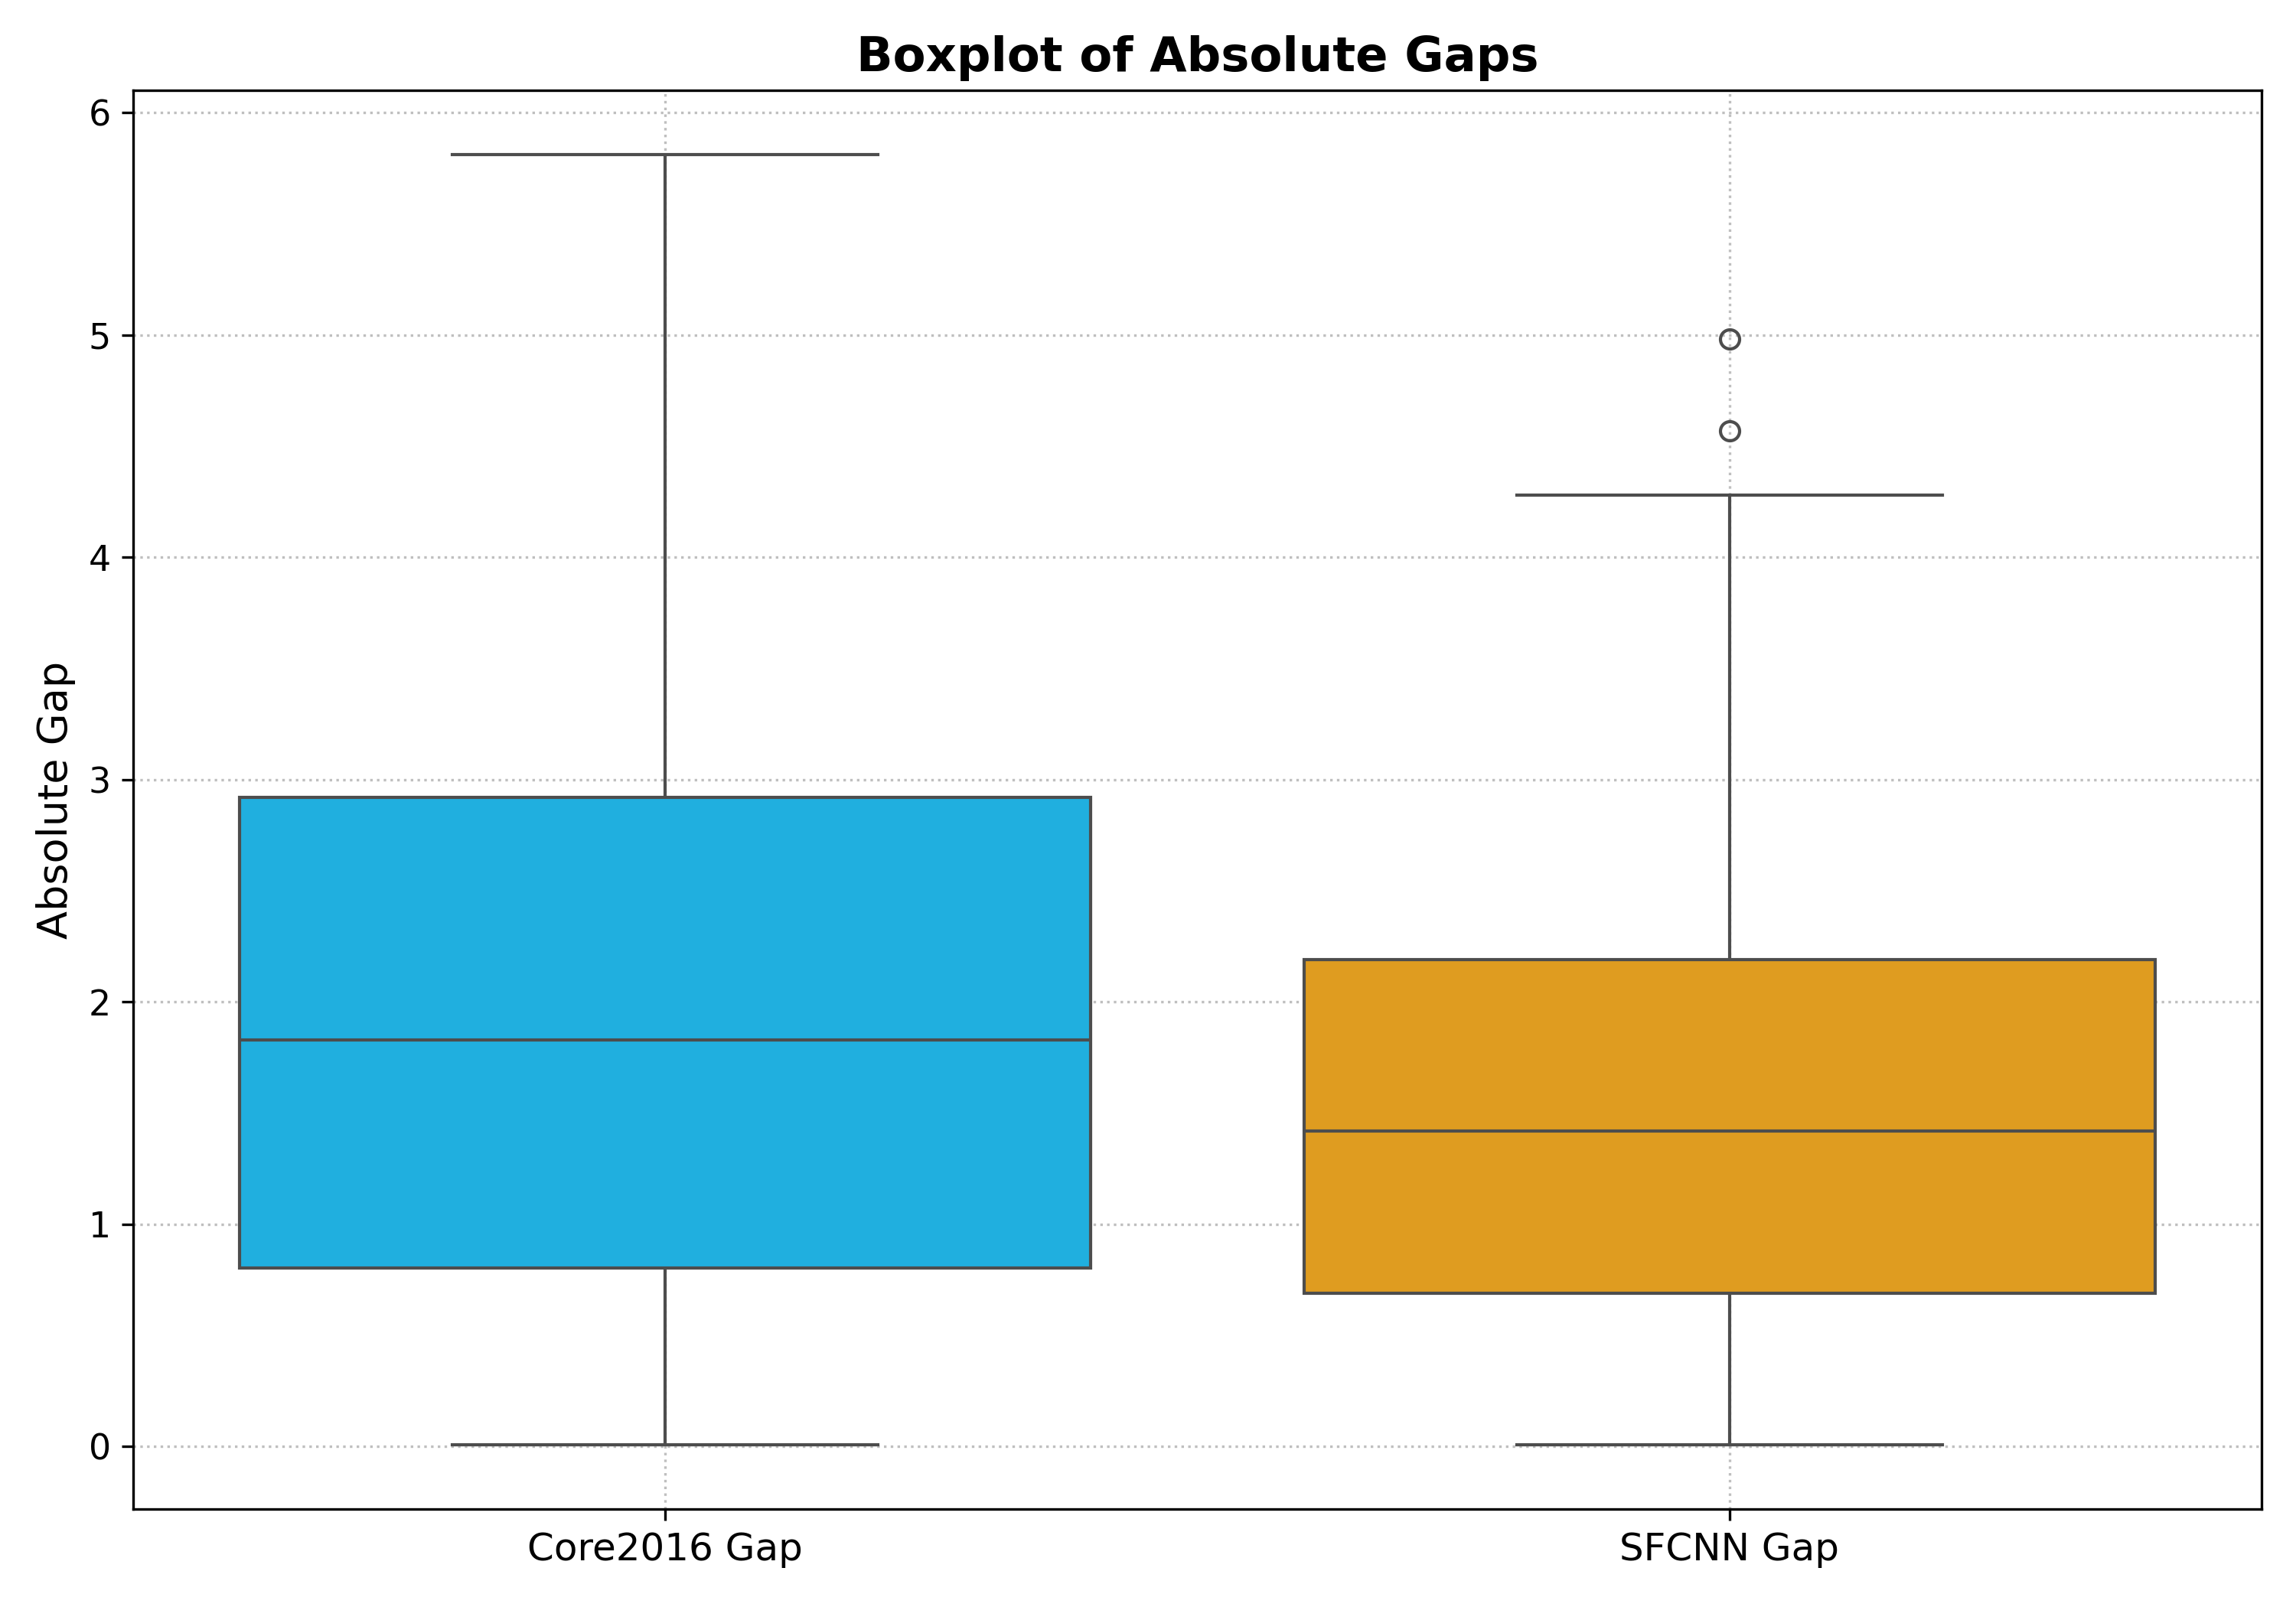
\includegraphics[width=0.34\textwidth]{images/gap_boxplot.png}
    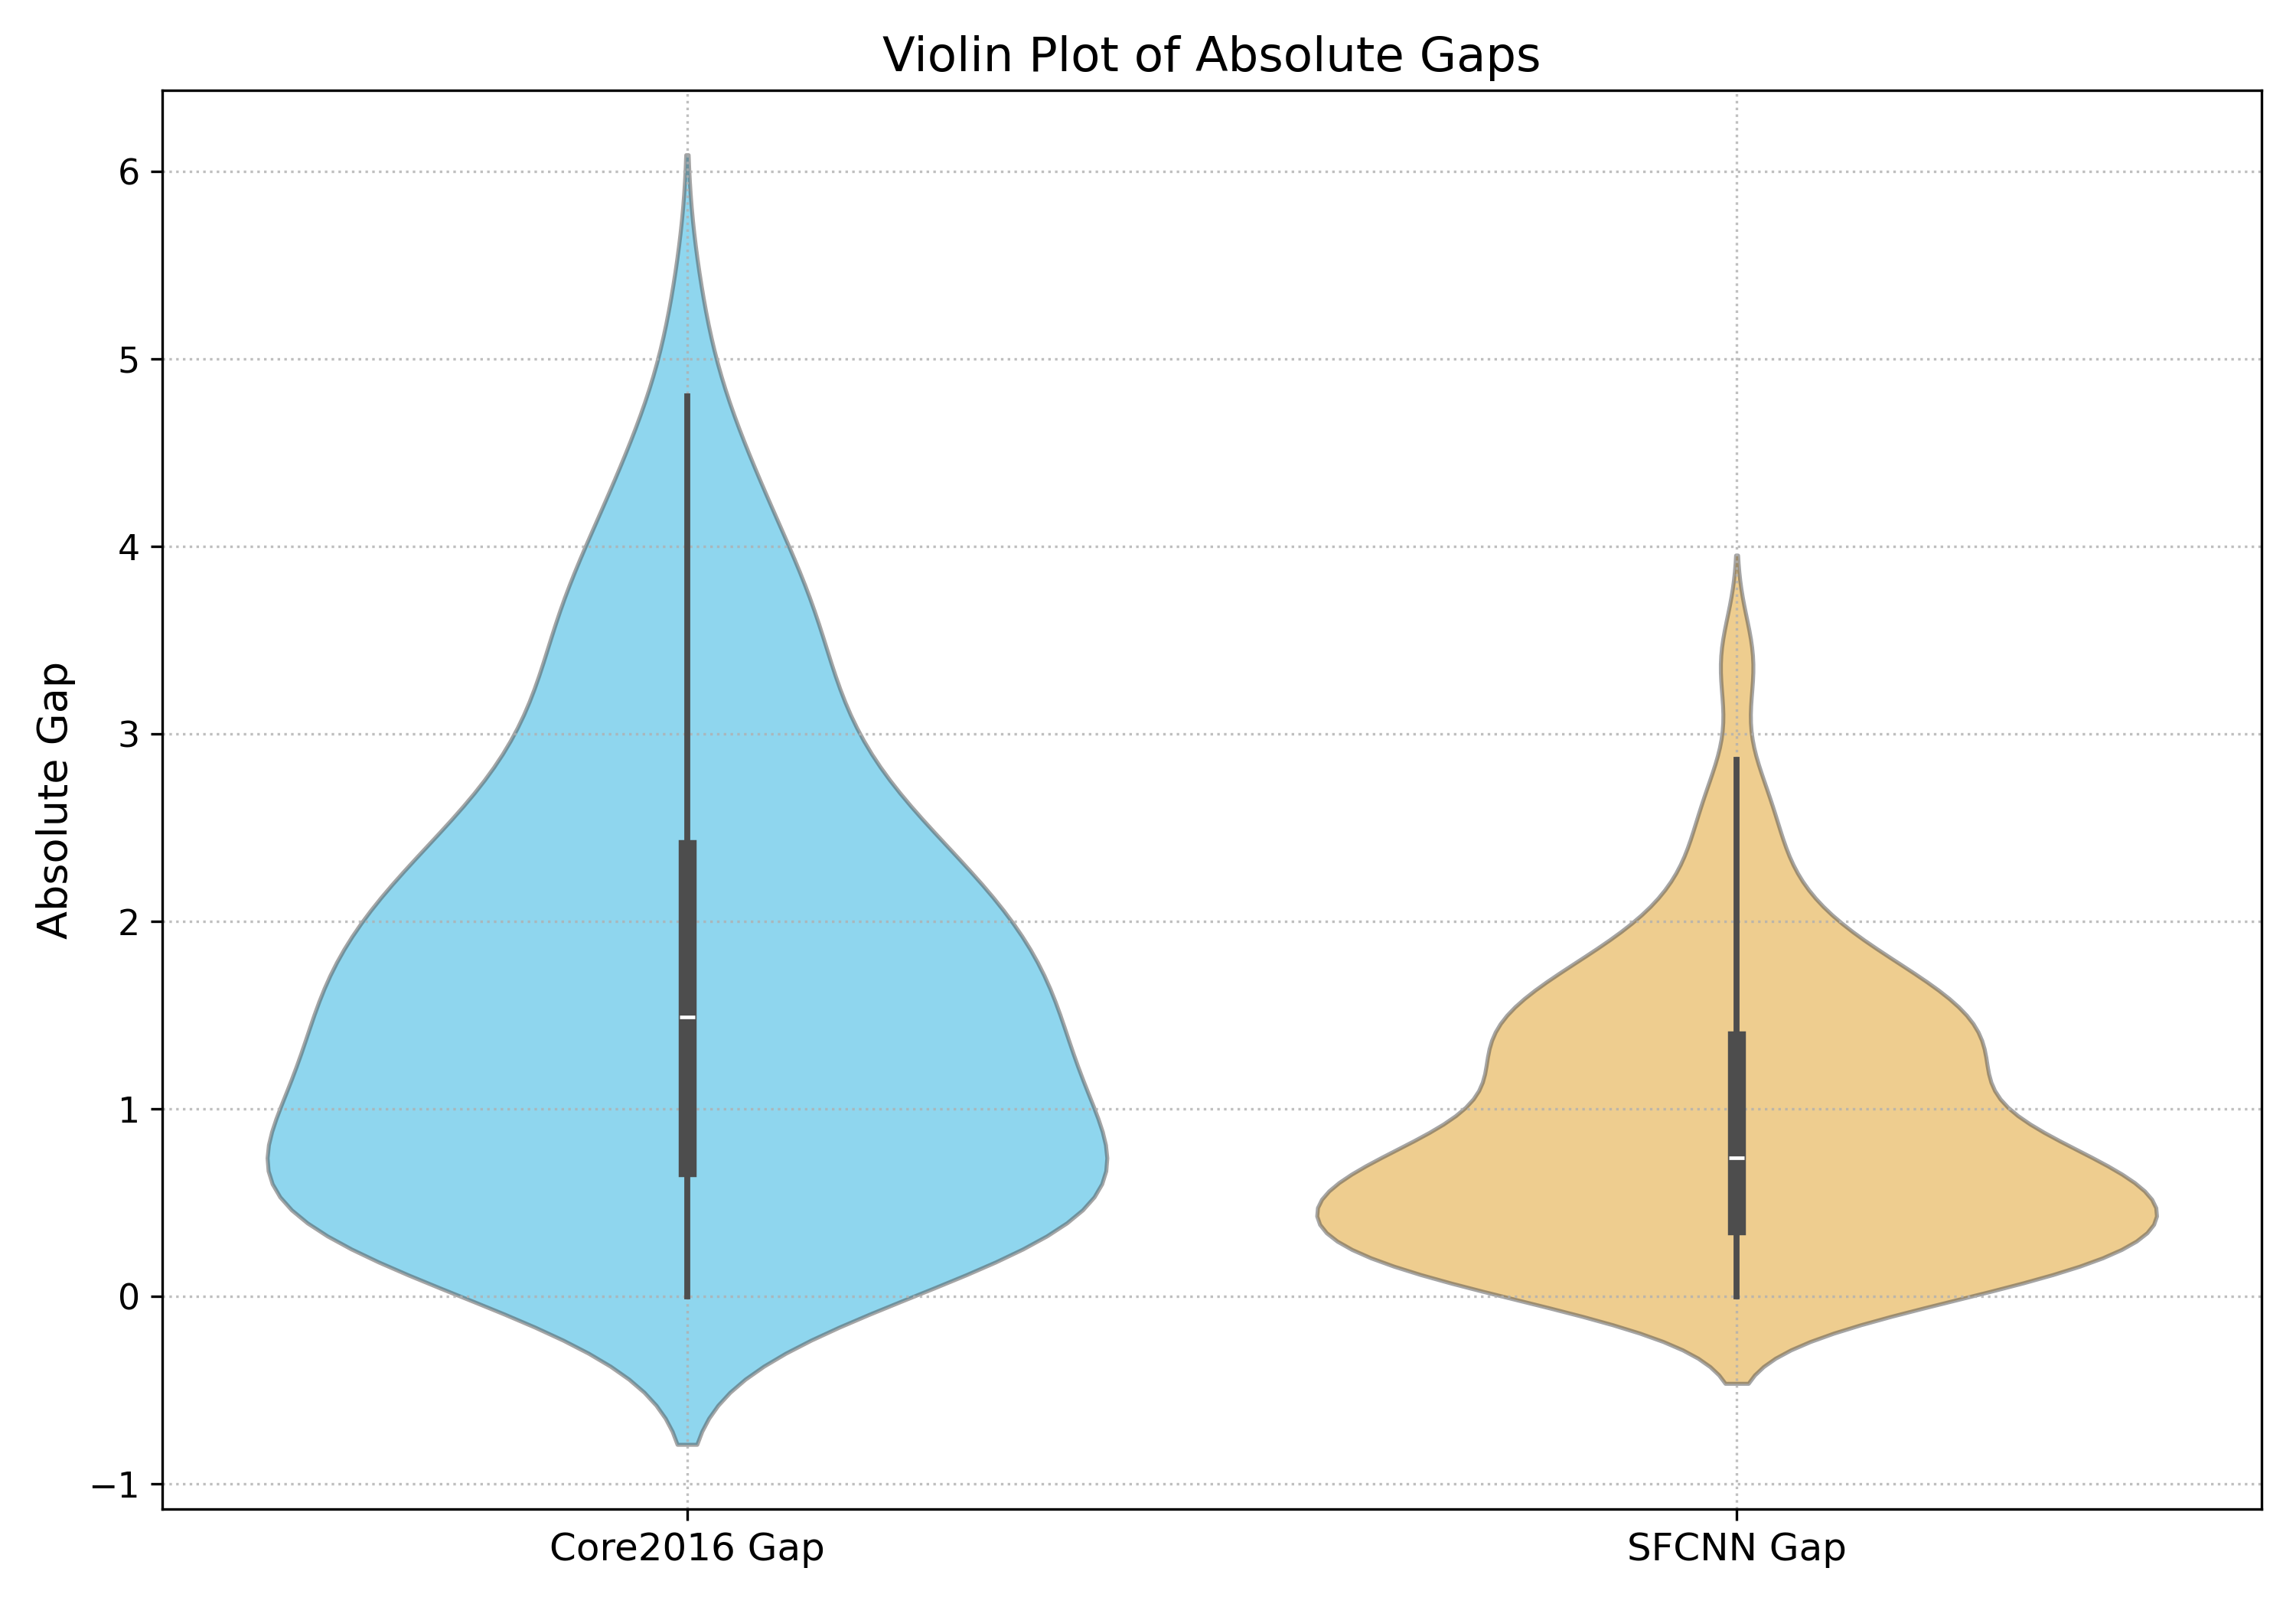
\includegraphics[width=0.34\textwidth]{images/gap_violinplot.png}
    \caption{Boxplot (left) and violin plot (right) of prediction gaps for AF3 structures.}
    \label{fig:af3_gap_box_violin}
\end{figure}

Figure~\ref{fig:af3_gap_box_violin} provides complementary perspectives: the boxplot summarizes the central tendency and spread, while the violin plot visualizes the full error distribution, emphasizing the presence of outliers and overall error landscape.

\subsection{Interpretation and Implications}
Collectively, these results demonstrate that while the reproduced Sfcnn model 
maintains moderate agreement with experimental affinities on the CASF-2016 core set, 
its predictive performance deteriorates when applied to AF3-predicted structures. 
The observed increase in RMSE and MAE, coupled with reduced correlation, 
indicates that current AF3 structural models introduce additional uncertainty into affinity 
prediction pipelines. Although AlphaFold3 is capable of generating plausible 
protein-ligand complex structures, its predictions are not yet sufficiently robust for 
quantitative PLA prediction using state-of-the-art deep learning scoring functions.

\subsection{Hypotheses for AF3's Reduced Performance}
The observed decrease in PLA prediction accuracy for AF3-generated structures may be attributed to two main factors:

\begin{enumerate}
    \item \textbf{Protein Structure-Specific Limitations:} Certain proteins in the CASF-2016 core set may possess structural features—such as large multimeric assemblies, flexible or disordered regions, or unusual binding site conformations—that challenge AF3's predictive capabilities. These cases can result in inaccurate modeling of the binding interface, leading to poor downstream affinity predictions.
    \item \textbf{AF3 Model and Dataset Constraints:} AlphaFold3 was primarily optimized for general protein and protein-ligand structure prediction, not specifically for quantitative affinity estimation. Its training data, loss functions, and architectural choices may not capture the subtle determinants critical for accurate PLA prediction. The lack of explicit optimization for binding affinity tasks may limit the transferability of AF3-generated structures to deep learning-based scoring functions such as Sfcnn.
\end{enumerate}

These hypotheses suggest that both target-specific structural challenges and broader methodological limitations of AF3 contribute to the observed performance gap. Future work could involve targeted analysis of outlier complexes and the development of structure prediction models tailored for affinity prediction tasks.

\section{Conclusion}
This study presents a systematic evaluation of AlphaFold3-predicted protein structures 
for protein-ligand affinity prediction using a reproduced Sfcnn model. 
The findings highlight the importance of reproducibility in deep learning models for 
structural biology and demonstrate the current capabilities and limitations of AF3 in 
the context of PLA prediction. 


\section{Author Contributions}

\subsection{Guo Yu}
\begin{itemize}
    \item Designed and implemented the data pipeline, including dataset curation, preprocessing, featurization, data augmentation, and storage.
    \item Managed exclusion of overlapping complexes and ensured data compatibility with the reproduced network.
    \item Designed and maintained the entire AF3 generation-evaluation workflow.
\end{itemize}

\subsection{Yiming Wu}
\begin{itemize}
    \item Implemented and reproduced the Sfcnn neural network architecture in PyTorch, adapting the original TensorFlow design.
    \item Designed and executed evaluation process for both experimentally determined and AF3-predicted structures.
\end{itemize}

\subsection{Yiyang Tan}
\begin{itemize}
    \item Conducted comparative studies and error analysis of model outputs, finished calculation of evaluation metrics (RMSE, MAE, SD, Pearson $R$).
    \item Generated all analysis visualizations, such as heatmaps, histograms etc..
\end{itemize}

\subsection{All Authors}
\begin{itemize}
    \item Contributed to the training process and hyperparameter tuning.
    \item Participated in the AF3 result generation.
    \item Participated in the interpretation of results and manuscript writing.
    \item Provided critical review of the paper and process.
\end{itemize}  

The project was conducted collaboratively with regular 
discussions to refine methodology and analysis.

\section{External Libraries}

\begin{itemize}
    \item \textbf{PyTorch}: Custom neural network implementation.
    \item \textbf{Pandas}: Data storage and analysis.
    \item \textbf{Numpy}: Data processing and manipulation.
    \item \textbf{Matplotlib}: Visualization of training loss curves.
\end{itemize}

\section{Acknowledgments}
This work was completed as the final project for the CS177: Bioinformatics—Software Development 
and Applications course at ShanghaiTech University. 
The authors thank the course instructors and teaching assistants 
for their guidance and support throughout the project.


\bibliographystyle{plain}
\bibliography{reference}

\end{document}